\chapter{Discussion - Patterns}
\section{Required Patterns}
	
\subsection{Observer}	
	\vspace{3 mm}
	\begin{multicols}{2}
	\paragraph{}
		The observer pattern defines a one-to-many dependency between objects so that when one object changes state all of its dependents are notified 
		about the change in state and update automatically. Creating highly coupled objects reduces their re-usability, so observer endeavors to 
		maintain the consistency among the collection of these cooperating classes. The subject or the object that has changed state invokes changes 
		on all the observers attached to it using the update method realized by the observer interface. This is done through the notify method in 
		the observable interface.
		\newline
		\newline
		As part of the community design, Observer in relation to Model View Controller would be used as a way to notify and update each clients views.  
		In this case the database on the distributors system.  A model adapter bound to the data source would receive an update via a notification as 
		a result to the change in the model.  Model changes would be propagate via the notification to a change to a view and the update operation 
		on the model would be executed.
		\newline
		\newline
		
		\begin{figurehere}
			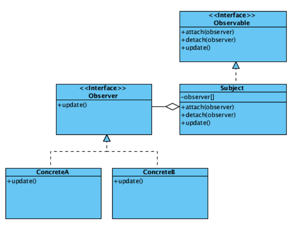
\includegraphics[scale=0.65]{figures/observer.png}
			\caption{Observer Design Pattern}
		\end{figurehere}
		
	\end{multicols}
\subsection{Factory Method}	
	\vspace{3 mm}
	\begin{multicols}{2}
	\paragraph{}
		The Factory Method Pattern defines an interface for constructing objects that lets subclasses decide which class to instantiate. It allows 
		the user to defer class construction to a subclass which is needed when a class can’t/shouldn’t be able to know which class of objects it 
		must construct i.e. the object construction ruses information or resources not appropriate for the composing object.
		\newline
		\newline
		The Creator isn’t bound to any Product class, it will work with any class that implements the Product Interface. Can cause unnecessary 
		sub classing e.g. we have Standard Team, and Three Team “Creators” for Three Player “Products”. Could have been avoided with templates 
		or delegates.
		\newline
		\newline
		\begin{figurehere}
			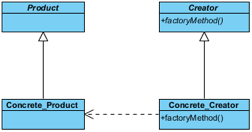
\includegraphics[scale=0.65]{figures/factory.png}
			\caption{Factory Method Design Pattern}
		\end{figurehere}
		
	\end{multicols}
	
\newpage
\subsection{Strategy}
	\vspace{3 mm}
	\begin{multicols}{2}
	\paragraph{}
		With the Strategy Pattern, we have different sets of behavior, similar in classification but different in implementation and we wish to 
		make them interchangeable. It allows the behavior of an algorithm vary independently from the object that uses it.
		\newline
		\newline
		Strategy allows us to group related algorithms but instead of having to subclass Context to give it different behaviors i.e. hard-wiring it, 
		we can abstract that behavior to allow us to vary the algorithm dynamically. Strategy allow avoids bloated conditionals in deciding which 
		behavior to use.
		\newline
		\newline
		The drawbacks of Strategy include its coupling to the client, as the Client must be aware of the strategies to decide which strategy to use.
		Similarly, the strategy will likely need data from context so you must either pass context to the strategy (when it may not use all of 
		Context’s data) or you may have to increase coupling between the context and strategies  to avoid too much unnecessary data being passed.
		\newline
		\newline
		In our case, Strategy worked well in allowed us to decide which AI moveset should be employed at run-time. It did force us however to pass 
		the data of which selected AI down through many objects that did not need to be aware of such things, an unfortunate consequence.
		\newline
		\newline
	\end{multicols}	
		
	\begin{figure}[h!]
		\centering
		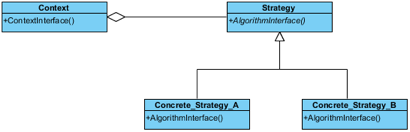
\includegraphics[width=100mm]{figures/strategy.png}
		  \caption{Strategy Design Pattern}
	\end{figure}
	
\subsection{Bridge}	
	\vspace{3 mm}
	\begin{multicols}{2}
	\paragraph{}
		The Bridge Pattern allows us to decouple abstraction and implementation so they be individually different. It is often considered to go 
		beyond encapsulation and be considered “insulation” (http://www.vincehuston.org/dp/ insulation.html). Often when implementations are 
		selected at run-time (what kind of display to use, in our project’s case) the implementation ends up very tied to its abstraction, which an 
		example of bad coupling and makes the product very complex. With Bridge we can change the implementation of the abstraction and have no 
		impact on the client.
	\end{multicols}	
		\begin{figurehere}
			\centering
			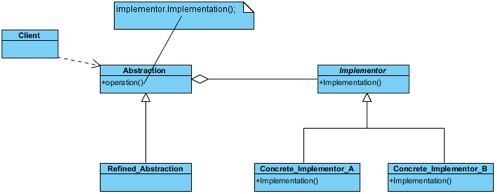
\includegraphics[width=140mm]{figures/bridge.png}
			\caption{Bridge Design Pattern}
		\end{figurehere}
	\begin{multicols}{2}
	\paragraph{}
		\vspace{8 mm}
		Obviously this allows us to extend Abstraction \& Implementor independently, so we’ve greater extensibility and we have greater encapsulation 
		because we can hide clients from implementation.
		\newline
		\newline
		In our project, we use Builder to separate the usage of the user interface from how it is implemented. This allows us to have the 
		abstracted functionality in the Game Window class, but have separate implementations of that functionality in Text\_Window \& 
		Model\_Window.
		\newline
		\newline
	\end{multicols}	
	
\subsection{Decorator}	
	\vspace{3 mm}
	\begin{multicols}{2}
	\paragraph{}
		The Decorator Pattern gives programmers an alternative to subclassing when wanting to add functionality to class, especially if one wishes to 
		do it dynamically.Extending without subclassing is particularly handy when there are a large number of possible/likely extensions as 
		subclassing would result in an enormous set of subclasses to support every combination. Decorator merely coats the existing object in one 
		with the extended functionality.
	\end{multicols}	
	
	\begin{figurehere}
		\centering
		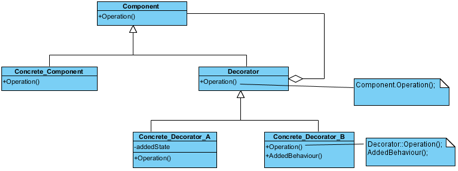
\includegraphics[width=120mm]{figures/decorator.png}
		\caption{Decorator Design Pattern}
	\end{figurehere}
	
	\begin{multicols}{2}
	\paragraph{}
		\vspace{8 mm}
		Decorator allows for dynamic growth of behavior rather than static inheritance.It also prevents use from subclassing every eventuality, 
		applications don’t need to “pay” for features they don’t use.  However Decorators are simply enclosures, a decorated component isn’t the 
		same as the component i.e. the object identity can be complicated, especially as another consequence of Decorator is that they will be many 
		small objects with different pieces of functionality (rather than one super object).
		\newline
		\newline
		In our project, Decorator is used to allow our concrete, or base map to have different kinds of obstacles on it e.g. mines. This avoids us 
		subclassing many different kinds and combinations of maps e.g. MinesMap, LandOMap, MinesAndLandOMap etc.
	\end{multicols}	

\section{Chosen Pattern}
\subsection{Memento}	

	\begin{multicols}{2}
	\paragraph{}
		Without violating encapsulation the memento pattern captures and restores an objects internal state. The memento pattern creates check points, 
		that let user back out or undo tentative operations.
		\newline
		\newline
		An obvious candidate for saving state and returning to a state is the memento pattern. The ability to undo or rollback and action is 
		advantageous not only to the end user but can reduce the load on a system. As part of the designing for concurrency and minimizing the 
		network traffic, one of the design patterns considered was the memento pattern. By using the pattern the current state could be stored 
		and restored later. 
	\end{multicols}	
		\begin{figurehere}
			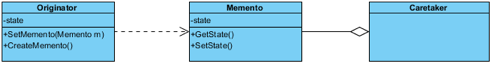
\includegraphics[scale=0.65]{figures/memento.png}
			\caption{Memento Design Pattern}
		\end{figurehere}
	\begin{multicols}{2}
	\paragraph{}
		\vspace{8 mm}
		By example when the user is browsing an online store, rather than re fetching the previous or next page the memento pattern can be used to 
		capture and externalize the previous objects internal state thereby implementing an undo mechanism but also reducing network load and the 
		interaction with the remote service. A checkout system is also a good candidate for this pattern as it would offer the user a rollback 
		mechanism in the case of an error and the ability to recover from a mistake without having to redo the entire sequence of operation that 
		led up to the undesired state.
		\newline
		\newline
		Another benefit of Memento is the avoiding of creating a direct interface to get an objects state which could expose implementation 
		details and thereby breaking encapsulation.
		\newline
		\newline
		However, the Memento Pattern does have certain drawbacks.  If the Originator has to copy large amounts of information to store in the 
		memento and/or the client is creating and replacing mementos quite often then there will be considerable overhead that will likely 
		affect performance and reliability. Generally one should avoid the Memento pattern unless encapsulating and restoring Originator 
		states is cheap.
		\newline
		\newline
		Similarly, depending on the size of the Memento, the caretaker might have a large storage cost when it stores mementos.
		On the issue of encapsulation, certain languages make it difficult to ensure only the originator can access the memento’s state, 
		being an issue with defining narrow/wide interfaces. By this I mean that the Caretaker sees a Narrow Interface (it can only pass 
		Memento to other objects) while the Originator sees a wide interface, so that it can access all the data needed to restore itself 
		to its previous state.
		\newline
		In our project Memento is used to allow the player to roll back after making a move. The Originator (the Player Object) has a “state” 
		which is its ship positions, which changes after every move. Before moving, the Caretaker (the Game Object) asks the player to create 
		a memento and stores it.
		\newline
		If after a player has moved (but during their turn) they click Undo, the Game Object will reset the state (in the Player Object) 
		to the memento previously created and delete that memento from its collection of mementos.
	\end{multicols}	
